% !TeX root = ../main.tex
% Add the above to each chapter to make compiling the PDF easier in some editors.

% as on http://tex.stackexchange.com/questions/89588/positioning-relative-to-page-in-tikz
% Defining a new coordinate system for the page:
%
% --------------------------
% |(-1,1)    (0,1)    (1,1)|
% |                        |
% |(-1,0)    (0,0)    (1,0)|
% |                        |
% |(-1,-1)   (0,-1)  (1,-1)|
% --------------------------
\makeatletter
\def\parsecomma#1,#2\endparsecomma{\def\page@x{#1}\def\page@y{#2}}
\tikzdeclarecoordinatesystem{page}{
    \parsecomma#1\endparsecomma
    \pgfpointanchor{current page}{north east}
    % Save the upper right corner
    \pgf@xc=\pgf@x%
    \pgf@yc=\pgf@y%
    % save the lower left corner
    \pgfpointanchor{current page}{south west}
    \pgf@xb=\pgf@x%
    \pgf@yb=\pgf@y%
    % Transform to the correct placement
    \pgfmathparse{(\pgf@xc-\pgf@xb)/2.*\page@x+(\pgf@xc+\pgf@xb)/2.}
    \expandafter\pgf@x\expandafter=\pgfmathresult pt
    \pgfmathparse{(\pgf@yc-\pgf@yb)/2.*\page@y+(\pgf@yc+\pgf@yb)/2.}
    \expandafter\pgf@y\expandafter=\pgfmathresult pt
}
\makeatother


\chapter{Appendix}\label{chapter:appendix}

\section{User study documents}
The following four documents are the files that were provided in the respective user study as is
\begin{itemize}
\item Orientation document revision 1 (for user study \#{}1) and revision 2 (for user study \#{}2)
\item Survey form revision 1 and revision 2
\item Tutorial document revision 1 and revision 2
\item Documentation revision 1 and revision 2
\end{itemize}

\includepdf[pages=-, height=\textheight, pagecommand={\subsection{Orientation} DOCUMENT: Orientation \textbf{revision 1}}]{./Appendices/Orientation_UserStudy1_English.pdf}
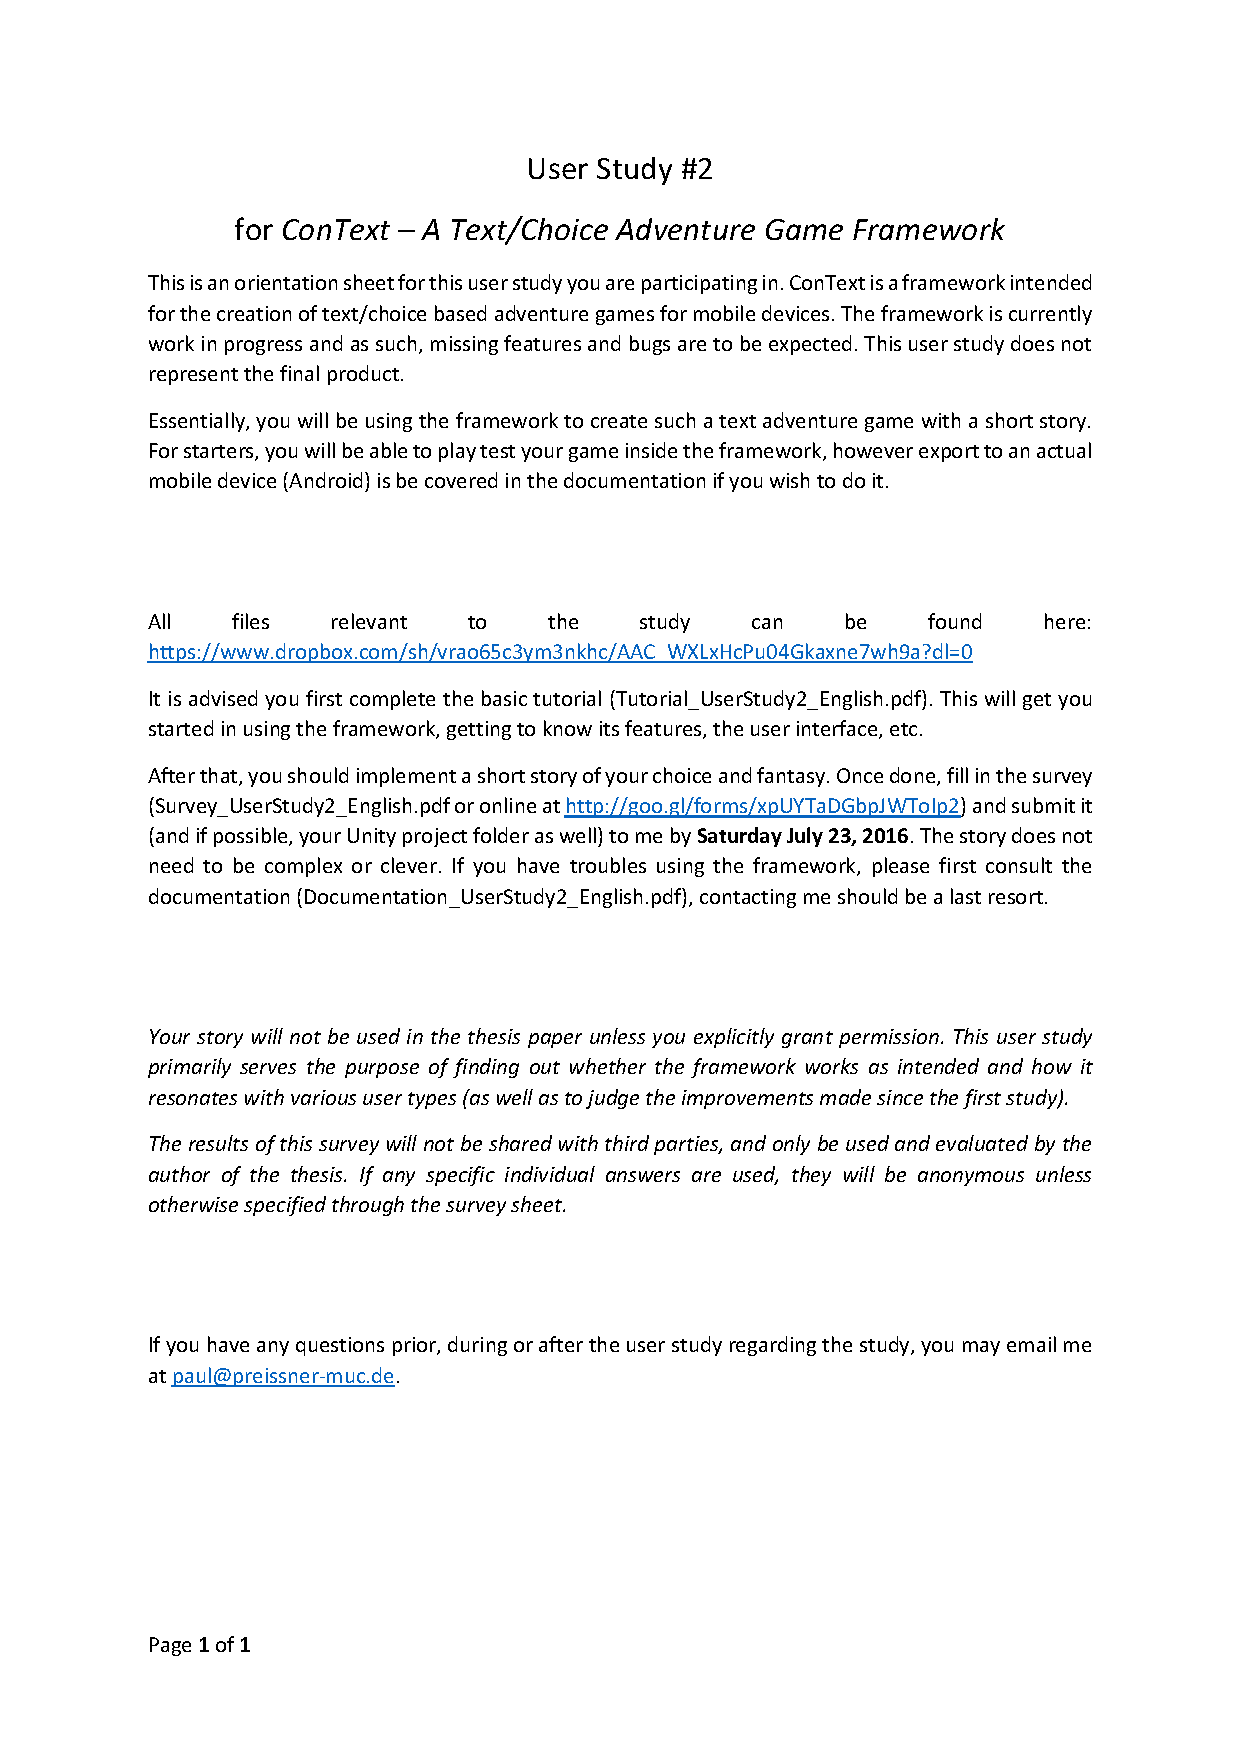
\includepdf[pages=-, height=\textheight, pagecommand={DOCUMENT: Orientation \textbf{revision 2}}]{./Appendices/Orientation_UserStudy2_English.pdf}


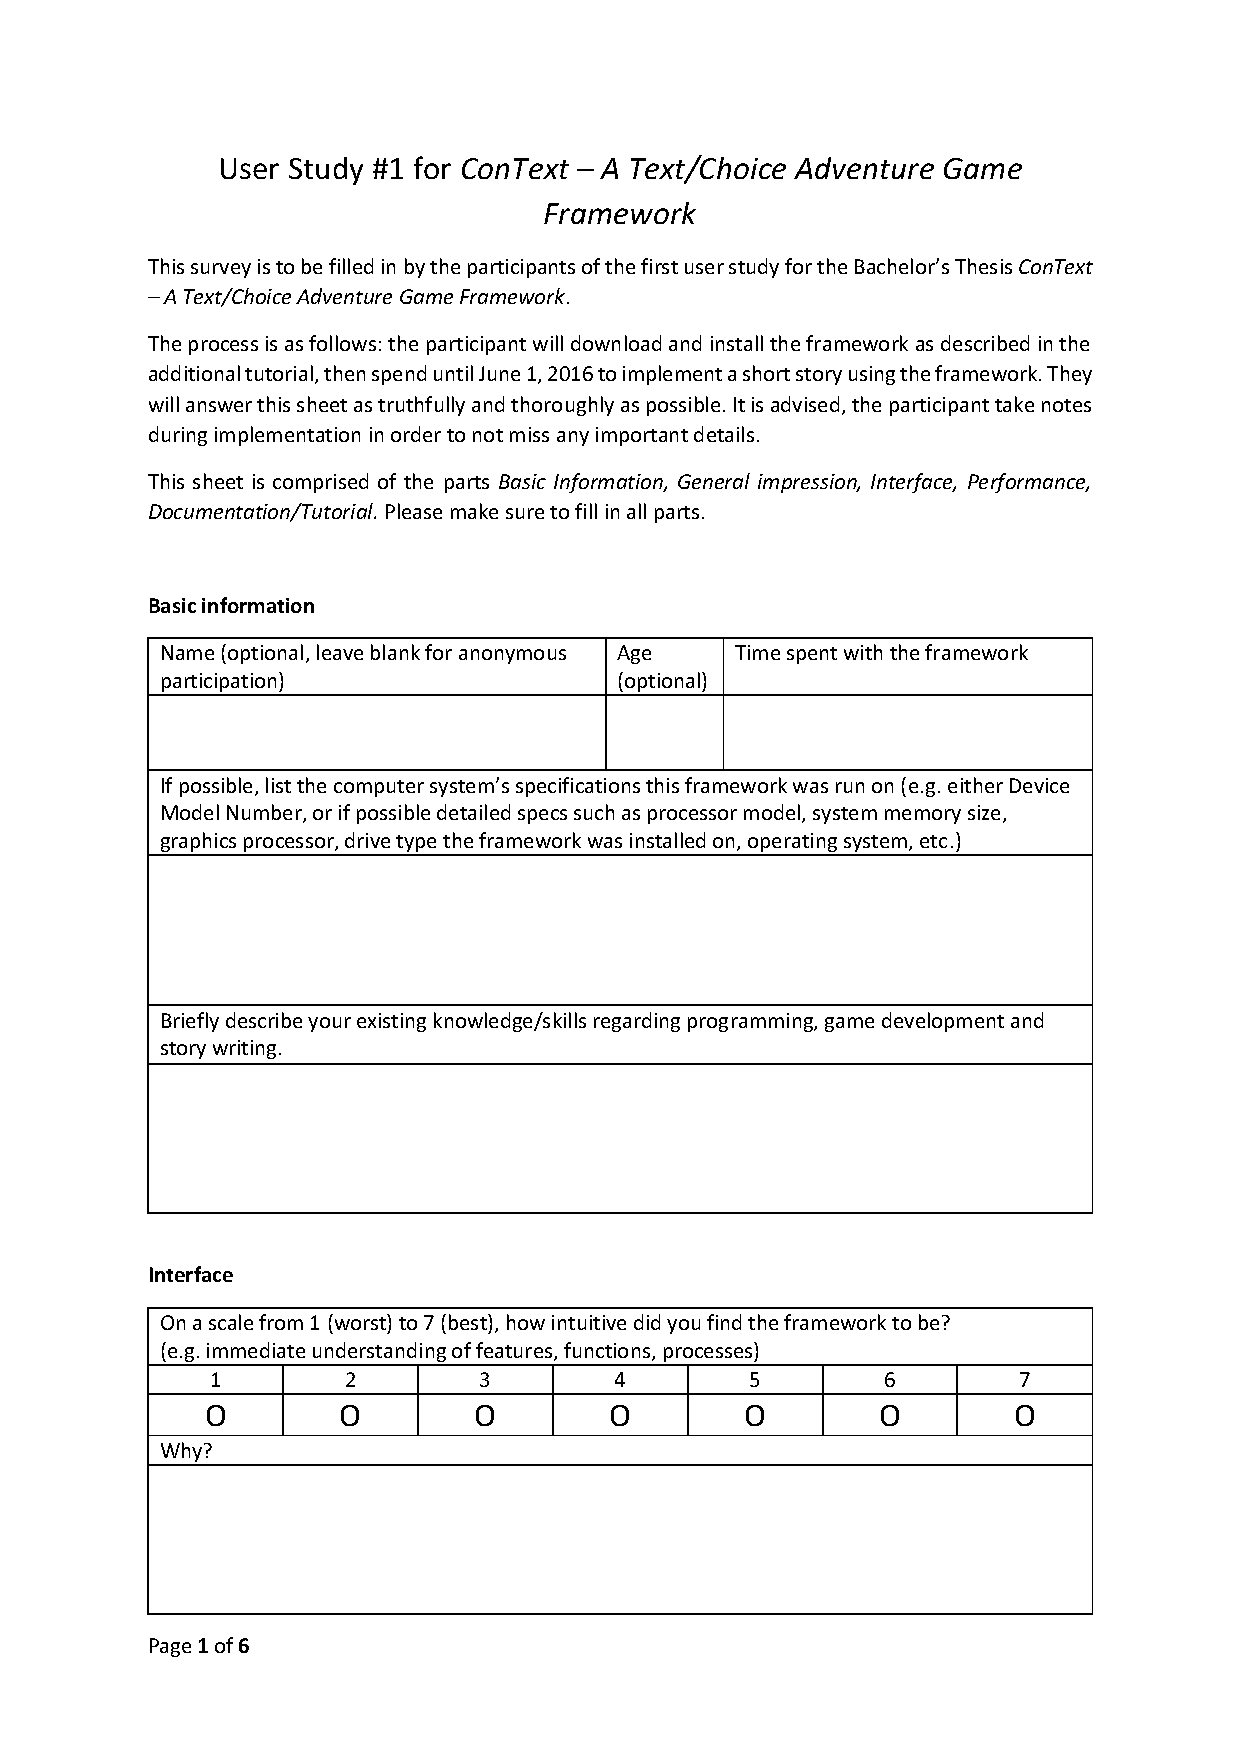
\includepdf[pages=1, height=\textheight, pagecommand={\subsection{Survey form} DOCUMENT: Survey form \textbf{revision 1}}]{./Appendices/ConText_UserStudy1_English.pdf}
\includepdf[pages=2-last, height=\textheight, pagecommand={DOCUMENT: Survey form \textbf{revision 1}}]{./Appendices/ConText_UserStudy1_English.pdf}
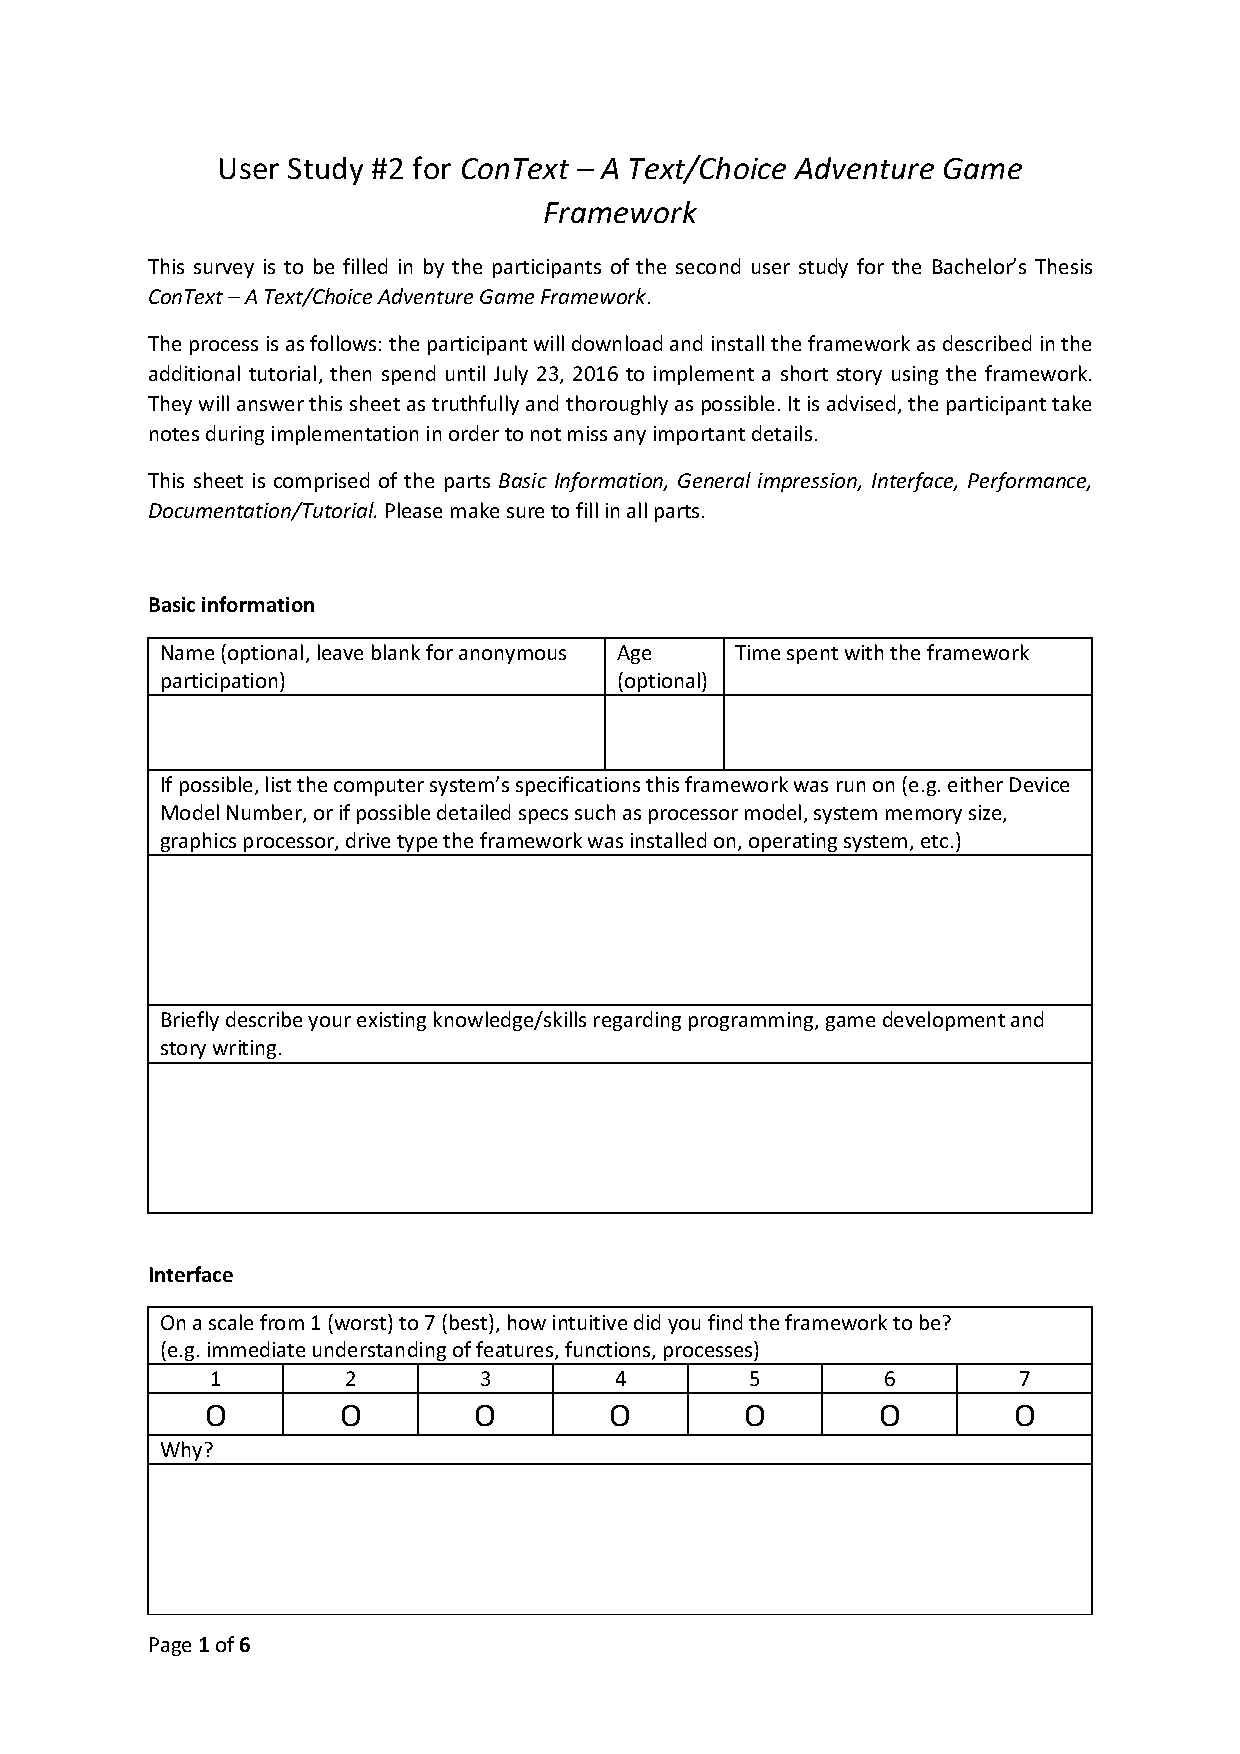
\includepdf[pages=-, height=\textheight, pagecommand={DOCUMENT: Survey form \textbf{revision 2}}]{./Appendices/ConText_UserStudy2_English.pdf}


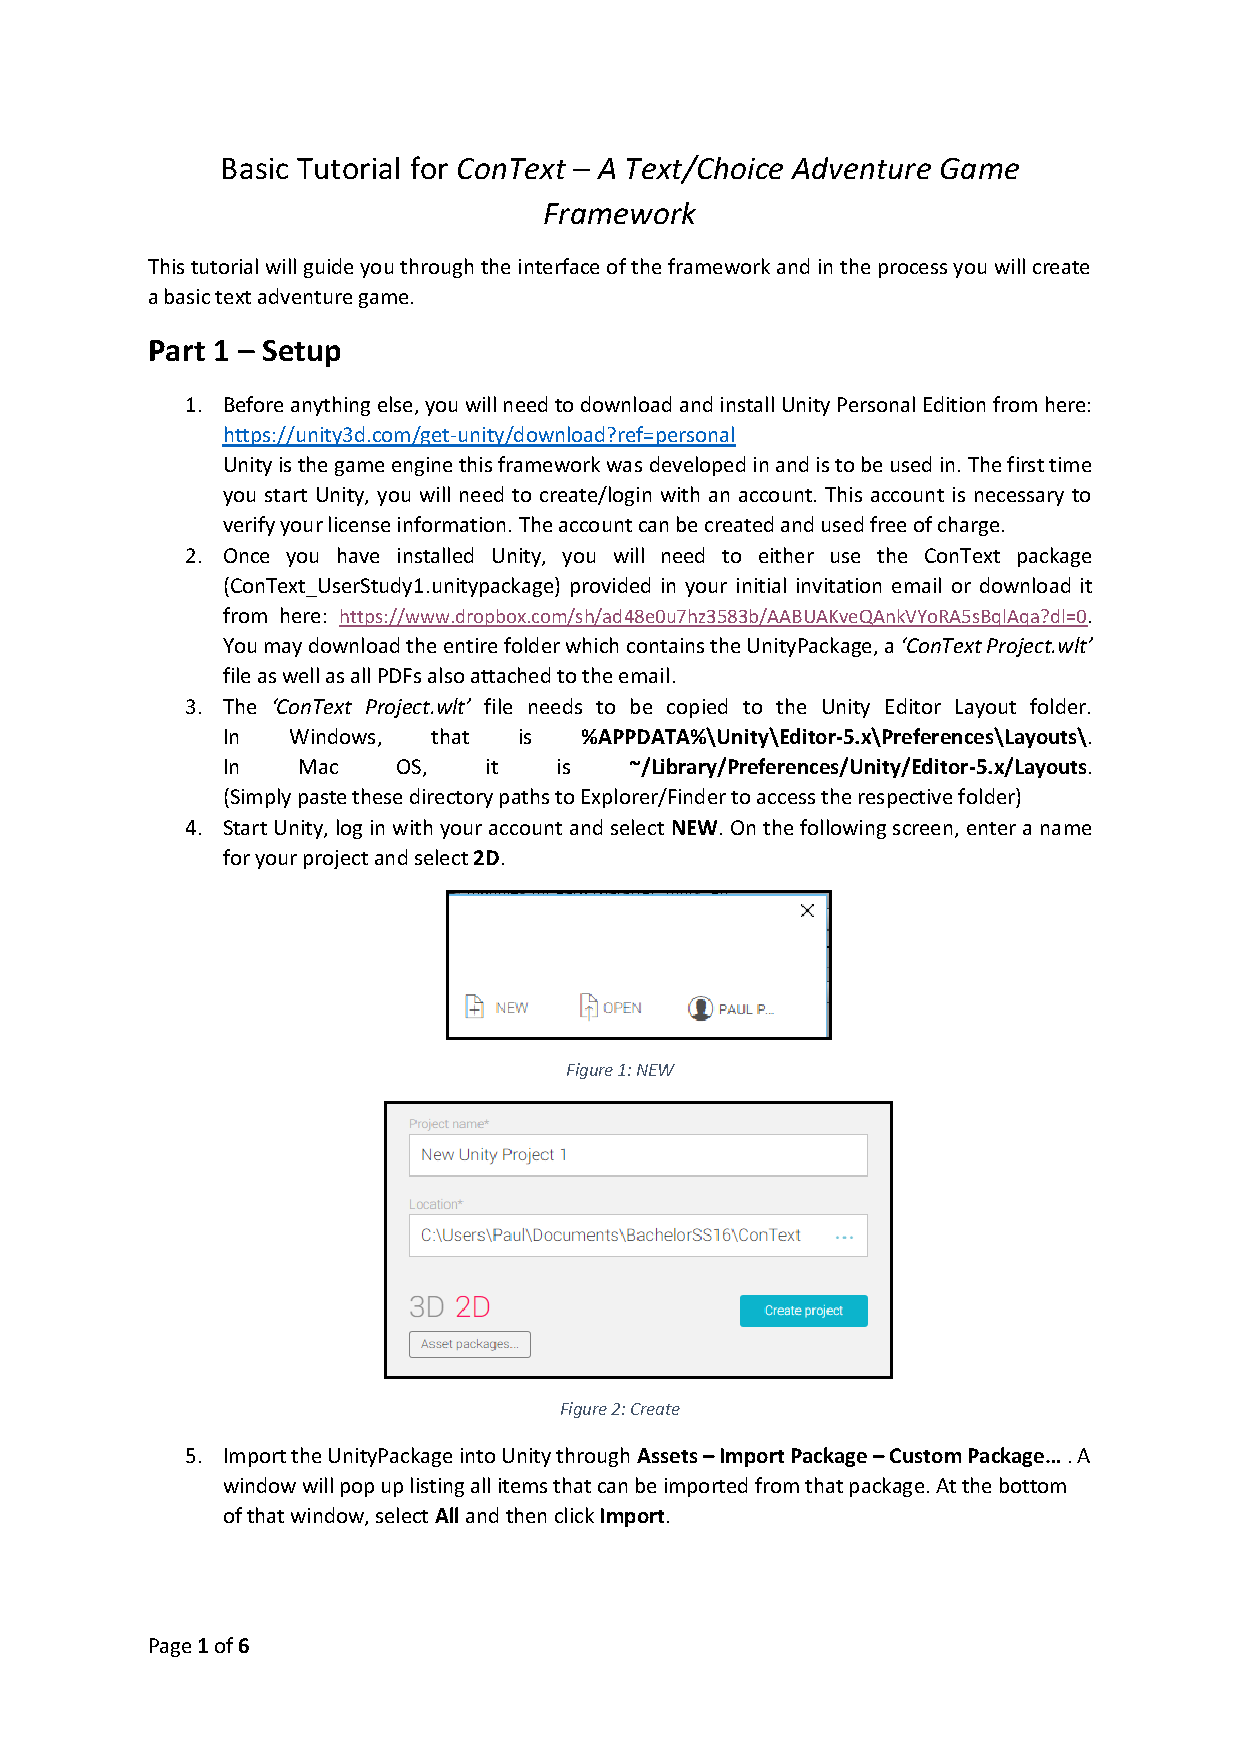
\includepdf[pages=1, height=\textheight, pagecommand={\subsection{Tutorial} DOCUMENT: Tutorial \textbf{revision 1}}]{./Appendices/Tutorial_UserStudy1_English.pdf}
\includepdf[pages=2-last, height=\textheight, pagecommand={DOCUMENT: Tutorial \textbf{revision 1}}]{./Appendices/Tutorial_UserStudy1_English.pdf}
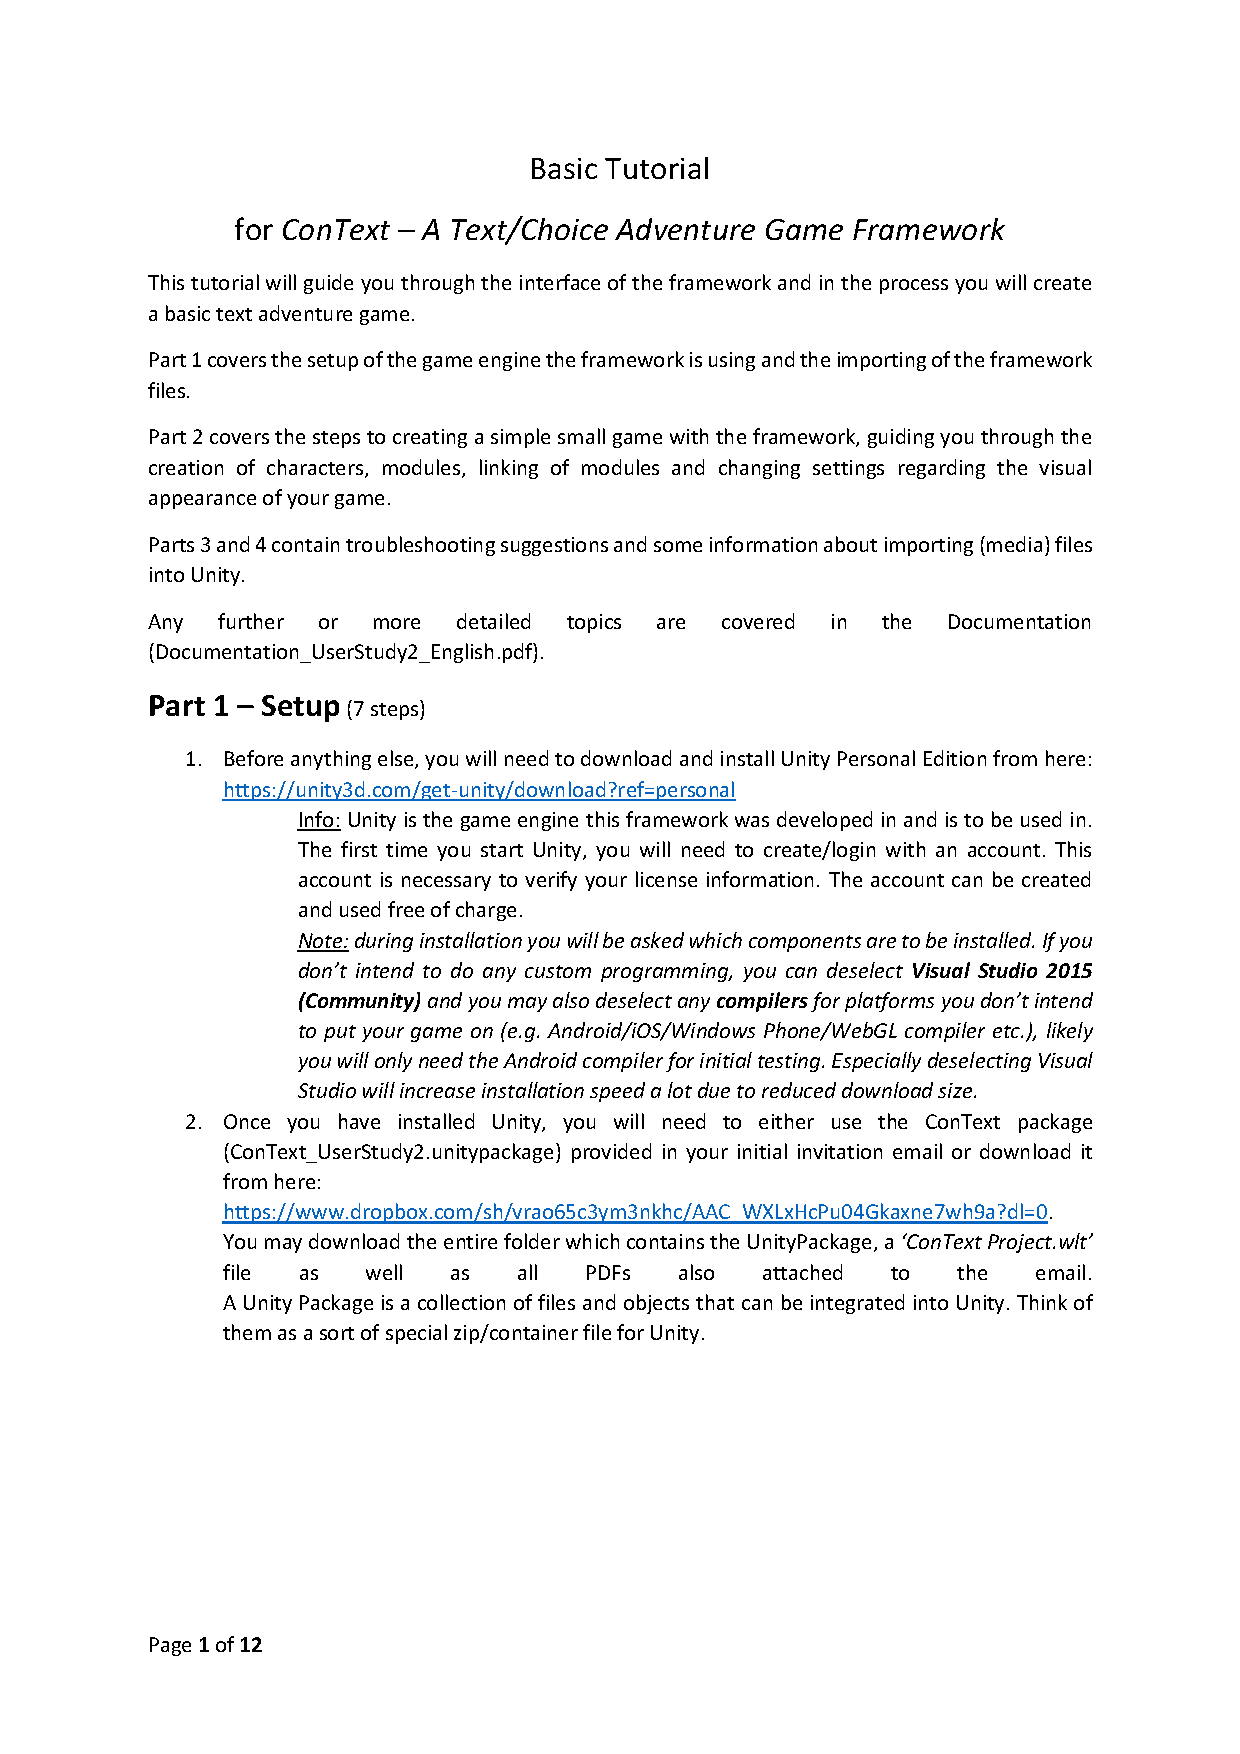
\includepdf[pages=-, height=\textheight, pagecommand={DOCUMENT: Tutorial \textbf{revision 2}}]{./Appendices/Tutorial_UserStudy2_English.pdf}


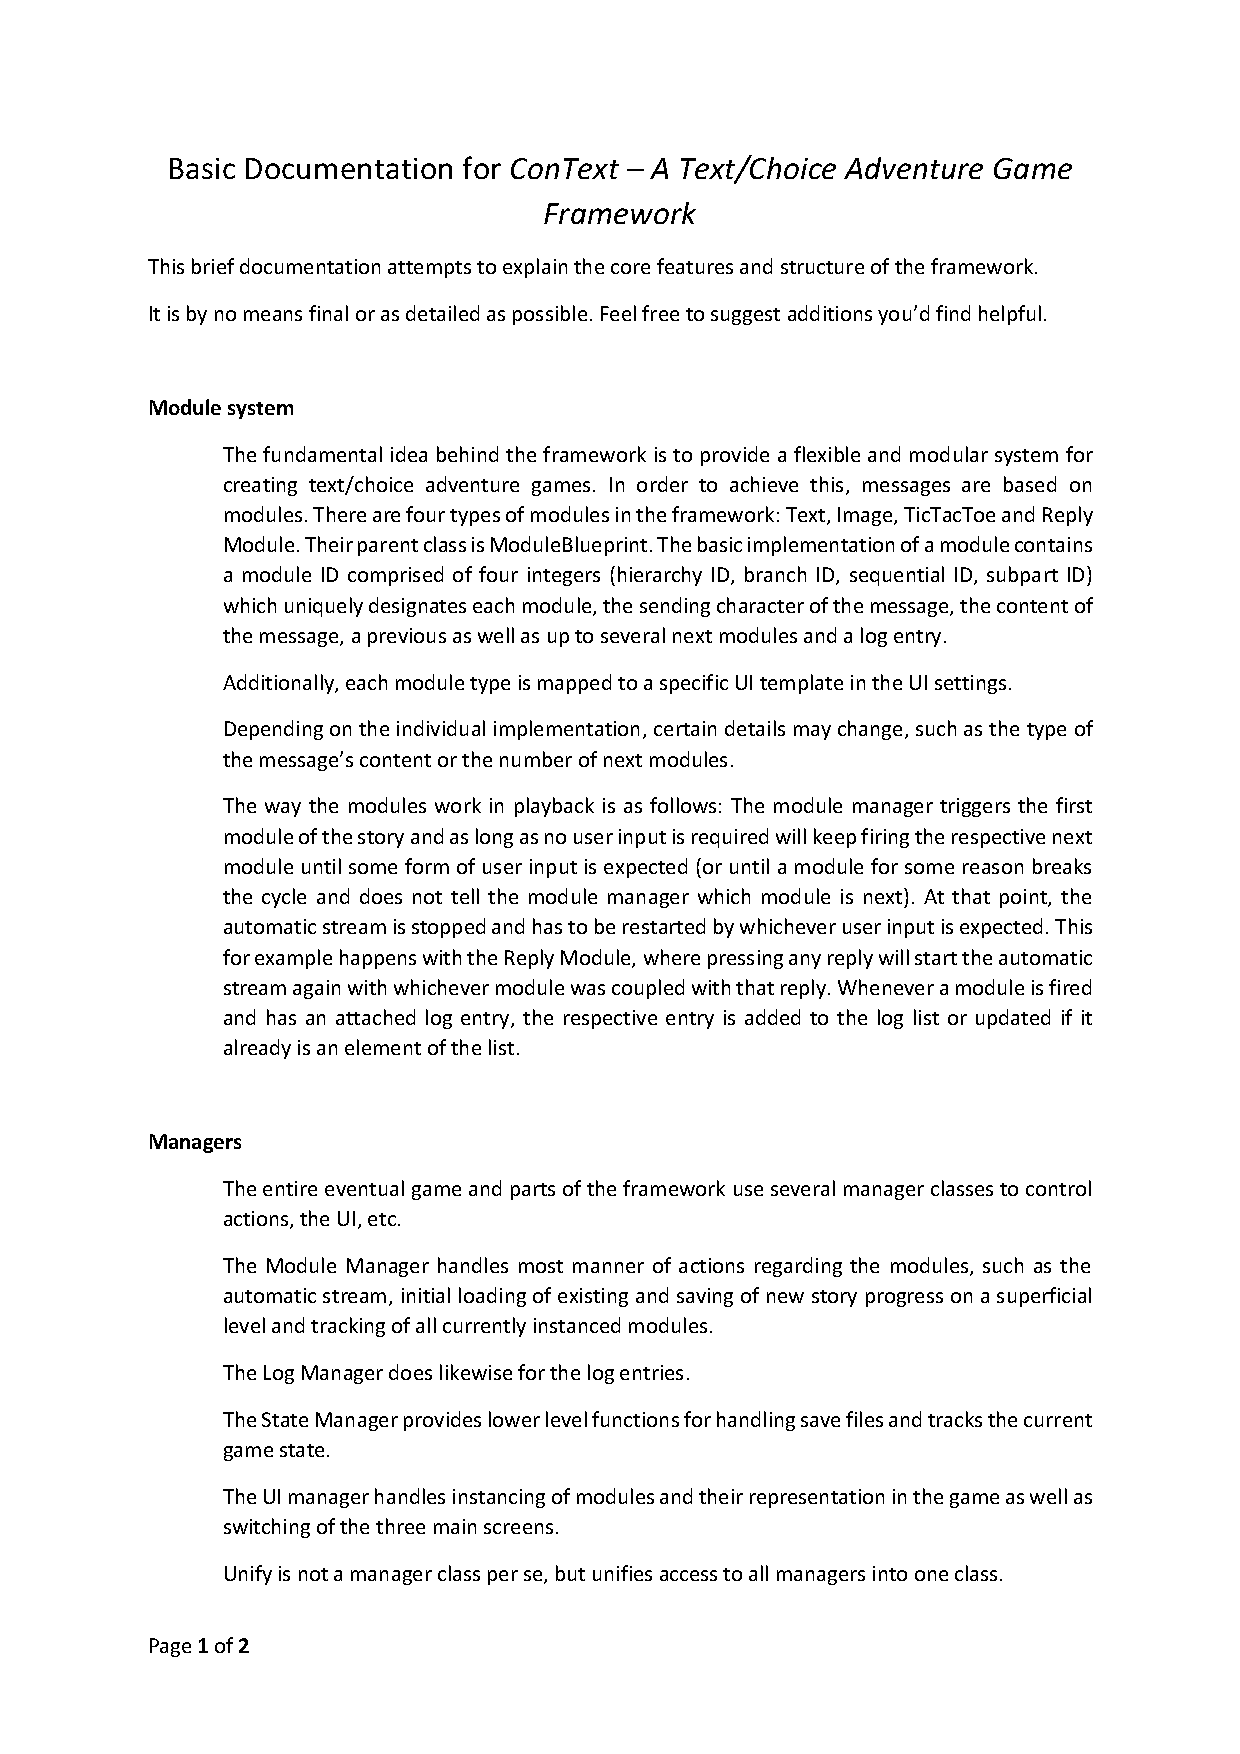
\includepdf[pages=1, height=\textheight, pagecommand={\subsection{Documentation} DOCUMENT: Documentation \textbf{revision 1}}]{./Appendices/Documentation_UserStudy1_English.pdf}\includepdf[pages=2-last, height=\textheight, pagecommand={DOCUMENT: Documentation \textbf{revision 1}}]{./Appendices/Documentation_UserStudy1_English.pdf}
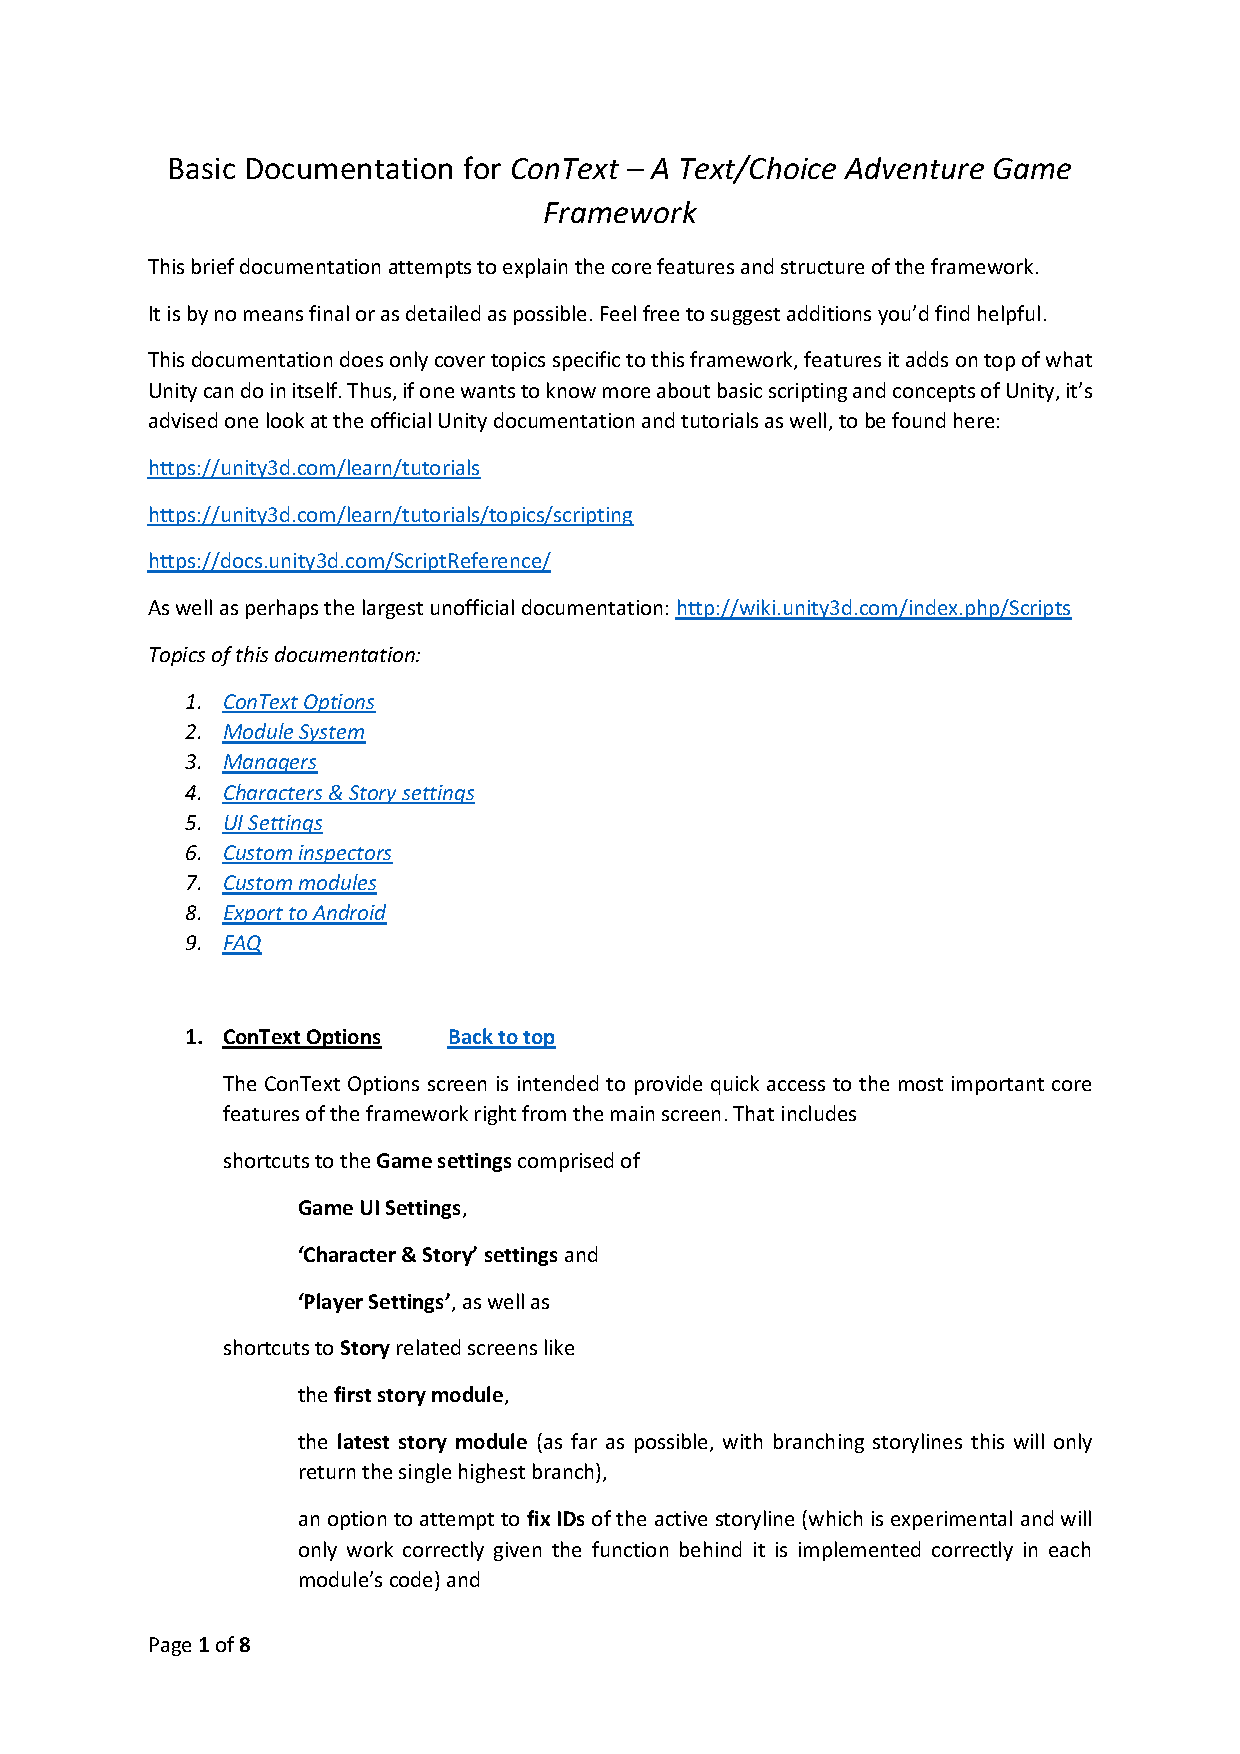
\includepdf[pages=-, height=\textheight, pagecommand={DOCUMENT: Documentation \textbf{revision 2}}]{./Appendices/Documentation_UserStudy2_English.pdf}

%\includepdf[pages=-, height=\textheight, pagecommand={\subsection{Orientation}\begin{tikzpicture}[remember picture, overlay]\node at (page cs:-0.5,0.73) {\textbf{ConText Orientation Revision 1}};\end{tikzpicture}}]{./Appendices/Orientation_UserStudy1_English.pdf}
%\includepdf[pages=-, height=\textheight, pagecommand={\begin{tikzpicture}[remember picture, overlay]\node at (page cs:-0.5,0.73) {\textbf{ConText Orientation Revision 2}};\end{tikzpicture}}]{./Appendices/Orientation_UserStudy2_English.pdf}